\documentclass[11pt]{tnetacle-en}

\lhead{tNETacle - English Document}
\rhead{}
\lfoot{}
\rfoot{}

\uptitle {Epitech Innovative Project}
\title {tNETacle}

\subtitle{English Document}
\date {}

\begin{document}

\member{Antoine Marandon}{ntnmrndn@gmail.com}
\member{Tristan Le Guern}{aversiste@gmail.com}
\member{Raphael Thoulouze}{raphael.thoulouze@gmail.com}
\member{Loïc Michaux}{loic.michaux@epitech.eu}
\member{Fabien Pichot}{pichot.fabien@gmail.com}
\member{Florent Tribouilloy}{tribouil@gmail.com}
\member{Nicolas Vivet}{nizzox@gmail.com}
\member{Pierre Wacrenier}{pierre.wacrenier@epitech.eu}

\summary{}

\maketitle

\fancyput(-2.54cm,-27.16cm){
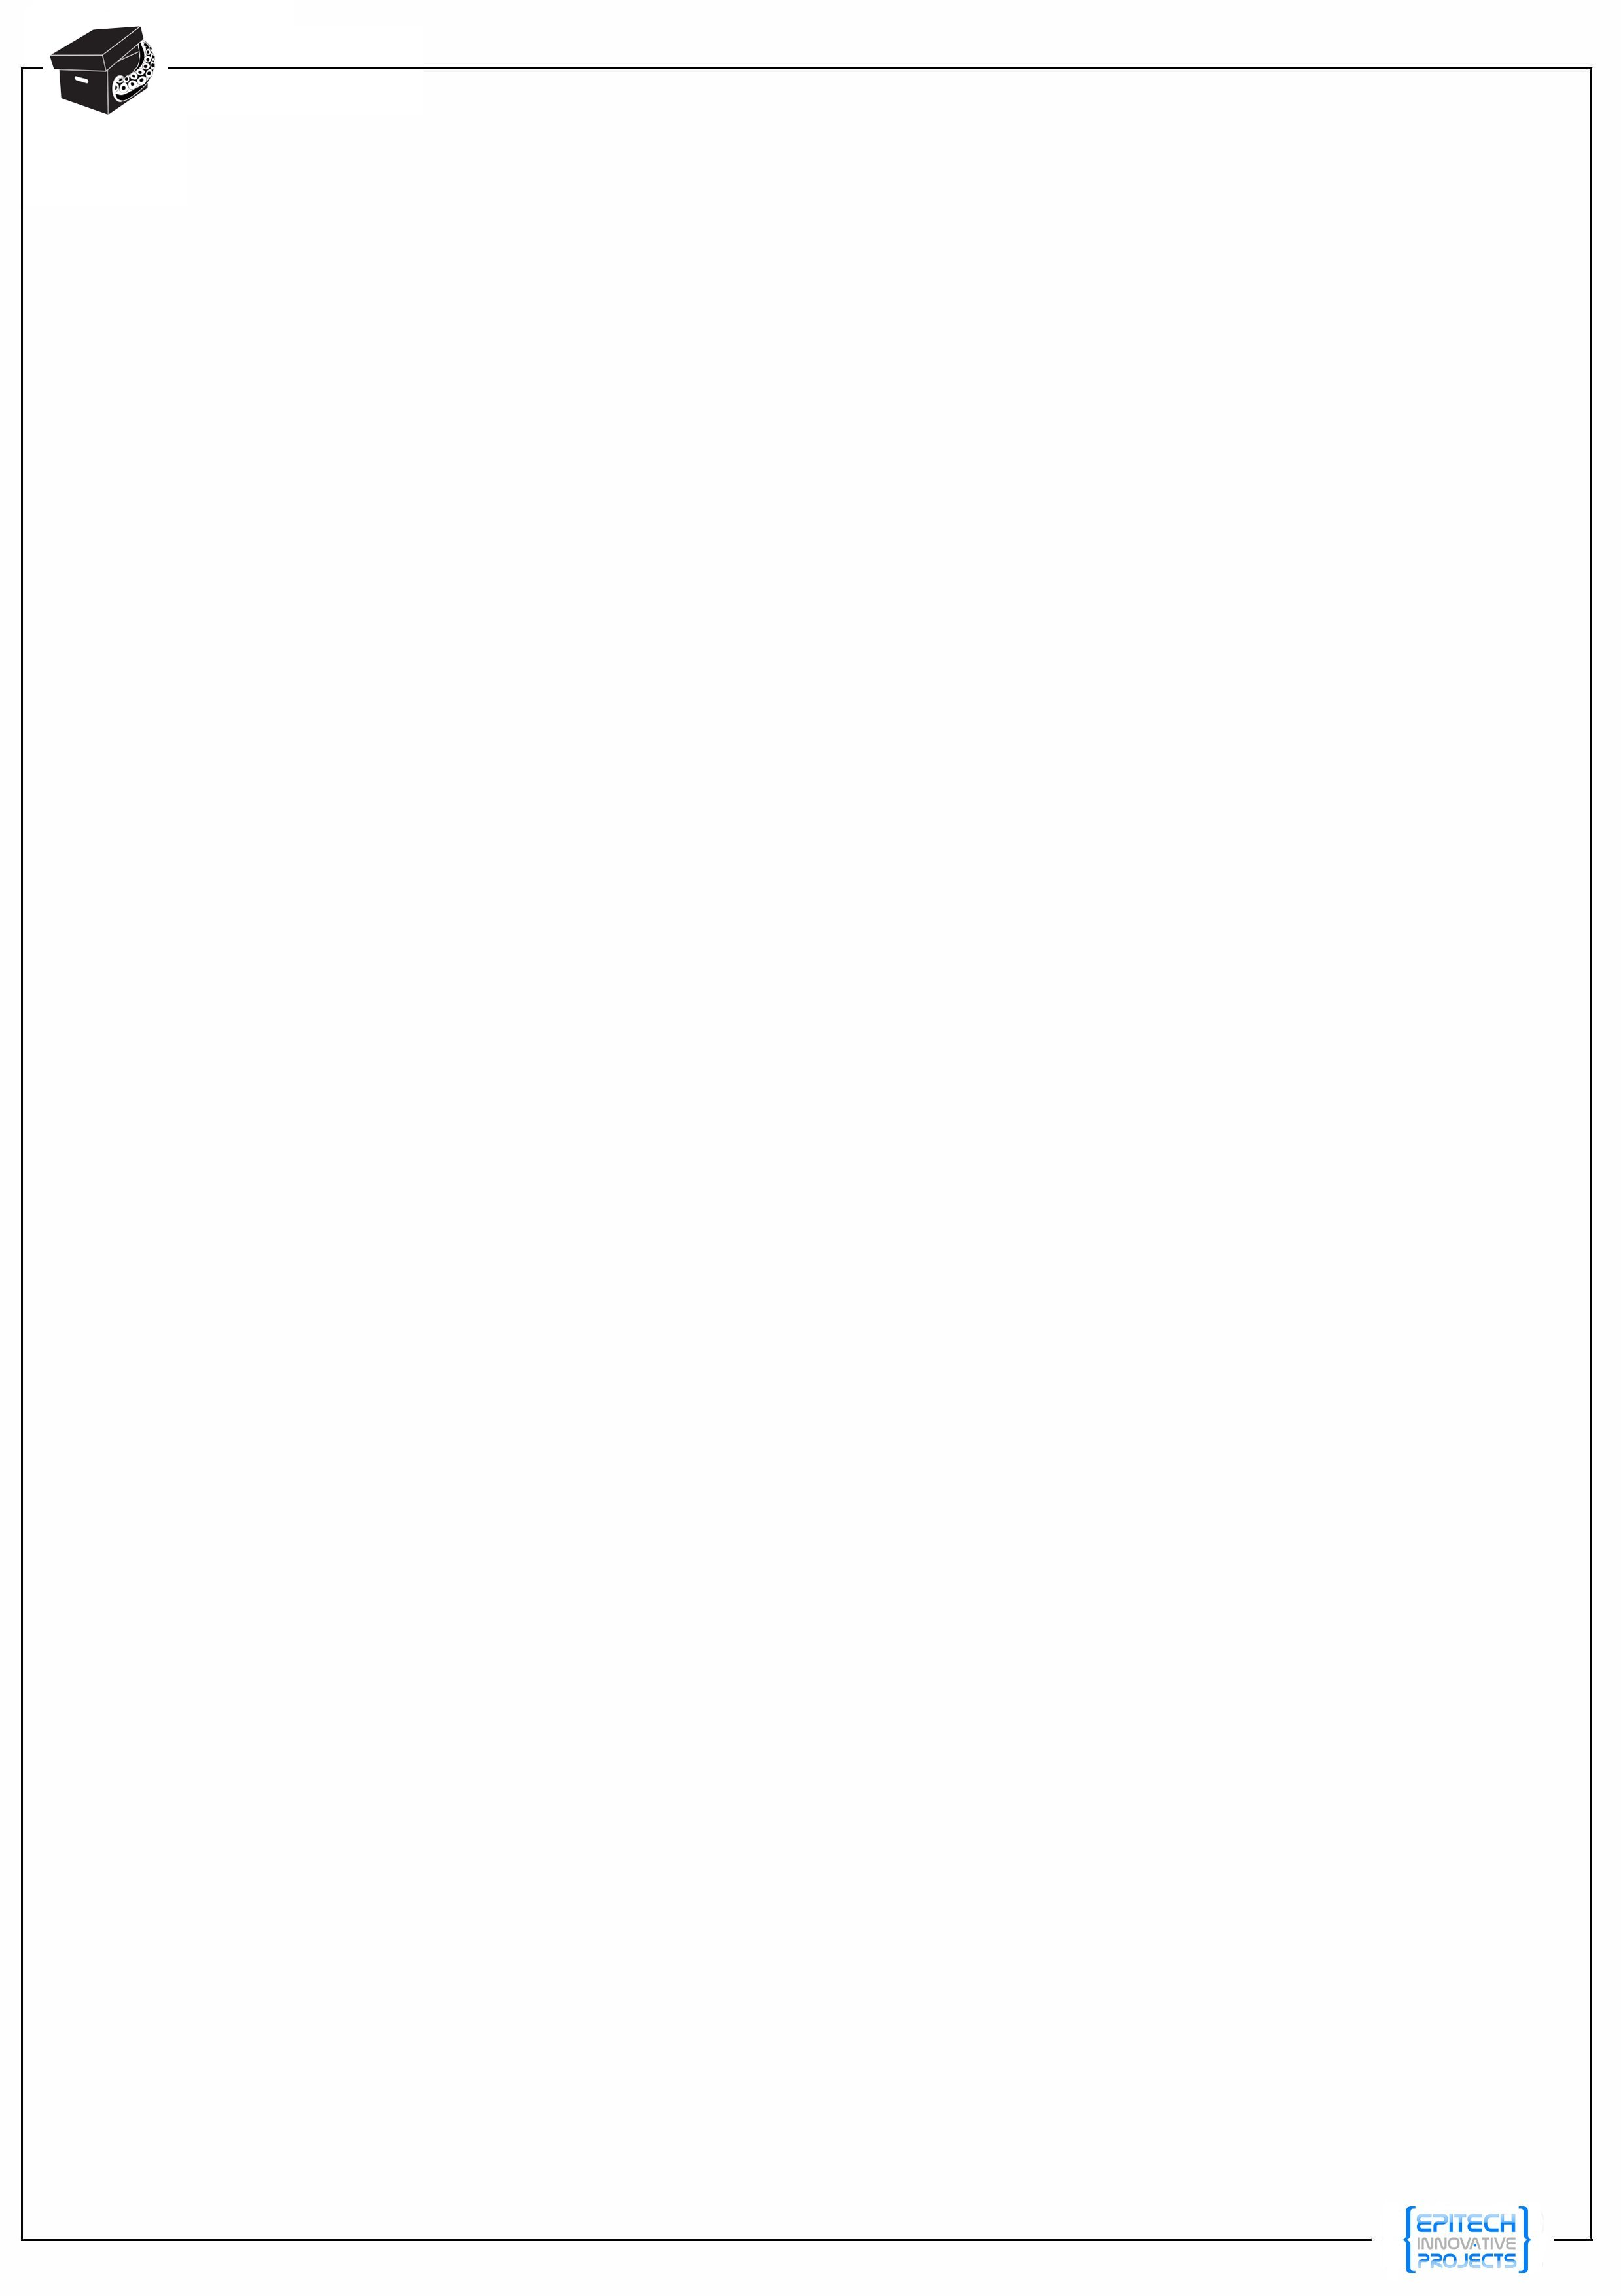
\includegraphics[width=21cm,height=29.7cm]{back-tnetacle-eip-bw.jpeg}
}

\begin{center}
\centerline{\Large\textsf{Revisions}}
\bigskip
\begin{tabular}{|c|c|l|}
\hline
Version            & Date       & Comments \\
\hline
0.0                & 2011-11-11 & revision comment \\
\hline
\end{tabular}
\end{center}
\clearpage

\tableofcontents

%\section{First section}
%\subsection{Subsection}

\end{document}
